\documentclass{beamer}



%%Beamer-Thema 
%\usetheme{Madrid} 
%%\usetheme{Warsaw} 
%%\usetheme{Berkeley}
%%Fontencoding 
%\usepackage[T1]{fontenc}
%
% \begin{document}
% \begin{frame}
%   \frametitle{Titel der Folie}
%   \begin{itemize}
%     \item erstes Item 
%       \pause
%     \item Item nach der Pause
%   \end{itemize}
% \end{frame}
% \end{document}\documentclass[11pt]{beamer}

 \usetheme{Warsaw}
 
 \usepackage{mathrsfs}
 \usepackage{color}
% \usepackage{cases}
 
 %\usepackage{hyperref}
%\usepackage{csquotes}
%\usepackage{tikz} 
%\usetikzlibrary{shapes,arrows}
%\usepackage{chngcntr}
 
 \usepackage[utf8]{inputenc}
 %\usepackage[T1]{fontenc}
\usepackage[ngerman]{babel}
 \usepackage{amsmath}
 \usepackage{amsfonts}
 \usepackage{amssymb}
 \usepackage[export]{adjustbox} % loads also graphicx
 \usepackage{graphicx}
 \usepackage{mathtools}
 \usepackage{multimedia} 
 \usepackage{color}
 
 \author{Garnik Arutyunyan, Marcel Gerhard, Heinz-Ullrich Rings}
 \title[Modellierungspraktikum]{Viskoelastizität}
 %\setbeamercovered{transparent} 
 %\setbeamertemplate{navigation symbols}{} 
 %\logo{} 
 \institute{Johannes-Gutenberg Universität Mainz} 
 \date{09. Juli 2019} 
 %\subject{Theo 6b} 
 \begin{document}

 \definecolor{mygreen}{rgb}{0,0.75,0} 
 
  \setbeamercovered{transparent}
 
 \begin{frame}
 \titlepage
 \end{frame}
 
 \begin{frame}
 	\tableofcontents
 \end{frame}
% 
\section{Einleitung}
\begin{frame}
\frametitle{Rheologie}
\begin{itemize}
	\item Viskose Rheologie bei Modellierung der Dynamik vom heißem, konvektierenden Inneren der Erde
	\item Modellierung relativ kalter, elastischer Lithosphäre erfordert viskoelastische Rheologie
	\item heißes sublithosphärische Innere verhält sich wie viskoses Fluid
	\item Lithosphäre zeigt elastisches Verhalten  
\end{itemize}
	
\end{frame}
	
\begin{frame}
\frametitle{Maxwell-Rheologie}
 \begin{columns}
 \column{0.5\linewidth}
 \begin{itemize}
 	\item Besteht aus Feder und Dämpfungselement
 	\item Sofortige Verformung der Feder bei Belastung
 	\item Danach beginnt viskose Verformung
 \end{itemize}
Nach Entlastung:
\begin{itemize}
	\item Feder bewegt sich zurück
	\item Viskoser Anteil bleibt bestehen
\end{itemize}
\column{0.5\linewidth}
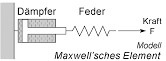
\includegraphics[scale=1]{images.jpg}
\end{columns}
\end{frame}
	

 \begin{frame}
 \frametitle{Viskoelastizität}
 Die viskoelastische Kraft kann hinsichtlich dreier Zeitintervalle aufgeteilt werden:
 \begin{enumerate}
 	\item instantane elastische Antwort
 	\item Relaxation der Scherkräfte auf der Zeitskala der Maxwell-Zeit
 	\item lineares Kriechen einer Newton'schen Flüssigkeit
 \end{enumerate}

\end{frame}

%\begin{frame}
%	\frametitle{Stokes Gleichungen für inkompressiblen Fluss}
%	\begin{align*}
%		&\int_{\Omega} B^T  D' B \bar{v}^{(k+1)} d\Omega -  %\int_{\Omega} B^T_{vol} H \bar{p}^{(k+1)} d\Omega -  %Ra\int_{\Omega}N^T N(T-T_0) \hat{z} d\Omega \\ &= 0
%	\end{align*}
%	\begin{align*}
%		\int_{\Omega}H^TB_{vol}\bar{v}^{(k+1)} d\Omega %-\frac{1}{\kappa} \int_{\Omega} H^T H \bar{p}^{(k+1)} d\Omega = - %\frac{1}{\kappa} \int_{\Omega} H^T H \bar{p}^{(k)} d \Omega
%	\end{align*}
%	$B, B_{vol}$: Ableitungen der Shapefunktionen \\
%	$N,H$: Shapefunktionen\\
%	$D'$: Rheologiematrix
%\end{frame}


\begin{frame}
	\frametitle{Stokes Gleichungen für inkompressiblen Fluss}
		\begin{align*}
			&\int_{\Omega} B^T \frac{2\mu \Delta t}{\Delta T + De\mu} D' B \bar{v}^{(k+1)} d\Omega -  \int_{\Omega} B^T_{vol} H \bar{p}^{(k+1)} d\Omega \\ 
			&-f  = -\int_{\Omega} B^T \frac{De\mu}{\Delta T + De\mu}(I+W)\tau^{*n}
		\end{align*}
		\begin{align*}
			\int_{\Omega} H^T B_{vol}  \bar{v}^{(k+1)} d\Omega = g
		\end{align*}
	$B, B_{vol}$: Ableitungen der Shapefunktionen \\
	$f, g$: externe Kraft und Randbedingungen
	$N,H$: Shapefunktionen\\
	$D'$: Rheologiematrix \\
	$W$: Jaumann Stress-Rotations-Matrix, mit 
	\begin{align*}
		W = 	\begin{bmatrix}
				0 & 0 & 2 \\
				0 & 0 & -2 \\
				-1 & 1 & 0 \\
				\end{bmatrix}
				B_{\omega} v \Delta t
	\end{align*}
\end{frame}

\begin{frame}
\frametitle{Stokes Gleichungen für inkompressiblen Fluss}
Matrixschreibweise der Stokes Gleichungen: \\
\par\medskip
$\begin{bmatrix}
K_{vv} & K_{vp} \\
K_{pv} & 0 \\
\end{bmatrix}
\begin{Bmatrix}
\bar{v}^{(k+1)} \\
\bar{p}^{(k+1)}
\end{Bmatrix}
= \begin{Bmatrix}
f \\
g
\end{Bmatrix}$
\par\bigskip
$K_{vv} = \int_{\Omega} B^T \frac{2\mu \Delta t}{\Delta T + De\mu} D' B \bar{v}^{(k+1)} d\Omega$ \\
\par\smallskip
$K_{vp} = \int_{\Omega} B^T_{vol} H \bar{p}^{(k+1)} d\Omega $ \\
\par\smallskip
$K_{pv} = K_{pv}^T$
\end{frame}


\begin{frame}
	\frametitle{Modellierung}
	inkompressibles viskoelastisches Material in 2D, mit dem Ansatz:
	\begin{align*}
		\epsilon (\nu) = \underbrace{\frac{1}{2\mu}\tau}_{viskos} + \underbrace{\frac{1}{2G}\frac{D\tau}{Dt}}_{elastisch}
	\end{align*}
	$\tau$: Spannungsdeviator, wobei $\sigma = -pI+\tau$ \\
	$\mu$: Viskosität \\
	$G$: Schermodul \\
	$\frac{D}{Dt}$: Objektive Zeitableitung
\end{frame}



\end{document}